\documentclass[a4paper,12pt]{article}
\usepackage{latexsym}
\usepackage{graphicx}
\usepackage{epsfig}
\usepackage{float}
\usepackage{natbib}
\usepackage{listings}
\graphicspath{{./}}
\DeclareGraphicsExtensions{.eps}
\author{Howard Kinsman}
\title{Computational Astrophysics Project 2 - Investigation of Stellar Orbits within Barred Spiral Galaxies}
\begin{document}
\maketitle
\section{Part 1}
The Fortran program orbit.f was used to solve the 2nd order differential equation of motion: 
\begin{equation} \label{motion}
   \frac{d^2\mathbf{r}(t)}{dt^2}=-\nabla\Phi\left(\mathbf{r}\right)-2\mathbf{\Omega_B}\times\mathbf{v}+\Omega_B^2\mathbf{r}
\end{equation}
where the gravitational potential of an elongated bar is represented by:
\begin{equation} \label{grav}
\Phi\left(x,y\right)=\frac{v_0^2}{2}ln\left(a^2+x^2+\frac{y^2}{q^2}\right)
\end{equation}
In order to solve a 2nd order equation it is necessary to first split it into two 1st order differential equations and solve for the x and y components:
\begin{equation} \label{dxdt}
\frac{dx}{dt}=v_x
\end{equation}
\begin{equation} \label{dvxdt}
\frac{dv_x}{dt}=\frac{-v_0^2x}{a^2+\frac{y^2}{q^2}+x^2}+2\Omega_B\frac{dy}{dt}+\Omega_B^2x
\end{equation}
\begin{equation} \label{dydt}
\frac{dy}{dt}=v_y
\end{equation}
\begin{equation} \label{dvydt}
\frac{dv_y}{dt}=\frac{-v_0^2y}{a^2q^2+q^2x^2+y^2}-2\Omega_B\frac{dx}{dt}+\Omega_B^2y
\end{equation}
\newpage
Equation \ref{dvxdt} was encoded into Fortran as:
\begin{lstlisting}
dydx(2) = (-v0**2*y(1))/(a**2+(y(3)**2/q**2)+y(1)**2)
         +2*om*y(4)+om**2*y(1)
\end{lstlisting}
Equation \ref{dvydt} was encoded as:
\begin{lstlisting}
 dydx(4) = (-v0**2*y(3))/(a**2*q**2+q**2*y(1)**2+y(3)**2)
         -2*om*y(2)+om**2*y(3) 
\end{lstlisting}

For the first run the initial conditions were set as $x=0$, $y=0.087$, $v_y=0$ and $v_x=-1.68$. The final time was set as 5 initially.
The accuracy of the integration was controlled by monitoring the Jacobi integral
which is conserved as a star moves in a rotating bar. An initial value for $\epsilon$ was set at $10^{-3}$. The plot of the Jacobi integral with time is shown in Fig. \ref{fig:jacobi1}. As can be seen it ranges from -.7747 to -.7738.

\begin{figure}[H]
\centering
\includegraphics[width=0.75\textwidth]{./Vx-1.68x5/jacobi1}
\caption{Plot of Jacobi integral with $\epsilon=10^{-3}$}
\label{fig:jacobi1}
\end{figure}

To improve accuracy the program was re-run with $\epsilon=10^{-5}$. Fig. \ref{fig:jacobi2} now shows a Jacobi integral values of -.774615 to -.774595, a substantial improvement.

\begin{figure}[H]
\centering
\includegraphics[width=0.75\textwidth]{./Vx-1.68x5/jacobi2}
\caption{Plot of Jacobi integral with $\epsilon=10^{-5}$}
\label{fig:jacobi2}
\end{figure}

Fig. \ref{fig:jacobi3} is a plot of the Jacobi integral this time where $\epsilon=10^{-7}$. This plot shows that most values of the integral hover around the -.774616 mark.
\begin{figure}[H]
\centering
\includegraphics[width=0.75\textwidth]{./Vx-1.68x5/jacobi3}
\caption{Plot of Jacobi integral with $\epsilon=10^{-7}$}
\label{fig:jacobi3}
\end{figure}

An attempt to further improve accuracy with values of $\epsilon=10^{-8}$ or $\epsilon=10^{-9}$ show that the accuracy actually starts to deteriorate - see Fig. \ref{fig:jacobi4}. Therefore a value of $\epsilon=10^{-7}$ was used for all subsequent runs of the program.

\begin{figure}[H]
\centering
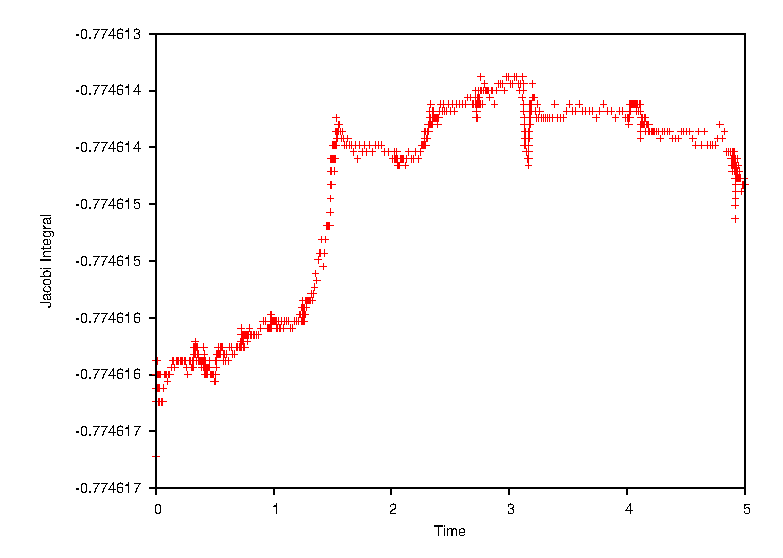
\includegraphics[width=0.75\textwidth]{./Vx-1.68x5/jacobi4}
\caption{Plot of Jacobi integral with $\epsilon=10^{-8}$}
\label{fig:jacobi4}
\end{figure}

Orbit trajectories were then calculated with a final time of 20. The first plot where $v_x=-1.68$ is shown in Fig. \ref{fig:orbit1}. The orbit is closed and has an elliptical shape. The star can be seen to be rotating around a bar-like shape. The plot also shows that the star does not orbit on a constant path, each subsequent orbit follows a slightly different path around the bar whilst maintaining the general elliptical shape. The path variations are greatest along the short axis.

\begin{figure}[H]
\centering
\includegraphics[width=0.75\textwidth]{./Vx-1.68x20/Graph2}
\caption{Plot of trajectory where $v_x=-1.68$}
\label{fig:orbit1}
\end{figure}

Figs. \ref{fig:orbit2} and \ref{fig:orbit3} show the same plots but with $v_x=-1.64$ and $v_x=-1.635$ respectively. The orbit here retains its essentially elliptical shape but the star now seems to orbit along a more constant path. This can be seen even more clearly in Fig. \ref{fig:orbit3} where subsequent orbits keep to the same general path around a bar-like shape. The orbit is also symmetrical about both the x and y axis.

\begin{figure}[H]
\centering
\includegraphics[width=0.75\textwidth]{./Vx-1.64x20/Graph2}
\caption{Plot of trajectory where $v_x=-1.64$}
\label{fig:orbit2}
\end{figure}

\begin{figure}[H]
\centering
\includegraphics[width=0.75\textwidth]{./Vx-1.635x20/Graph2}
\caption{Plot of trajectory where $v_x=-1.635$}
\label{fig:orbit3}
\end{figure}

Figs. \ref{fig:orbit4} to \ref{fig:orbit9} show the trajectory plots where the value of $v_x$ has values of -1.63, -1.58, -1.15, -.6, -.524 and -.4 respectivetly. They are again all closed orbits. As $v_x$ increases the orbits can be seen to gradually become more erratic. In Fig. \ref{fig:orbit5} the orbit begins to lose its elliptical shape and become slightly rounder but again showing the radius of the orbit varying widely along the shorter axis. Fig. \ref{fig:orbit6}, where $v_x=-1.15$, the orbits, although still surrounding a bar-like feature, no longer follow constant paths and the radial distance is not constant at any points. Further increases of $v_x$, as in Fig. \ref{fig:orbit7}, creates orbits which no longer orbit a bar-like shape, and takes on an almost torus-like shape with the star seeming to make small epicycles within the torus as it orbits the galaxy. When $v_x$ has been increased to -.524, as in Fig. \ref{fig:orbit8}, a more stable orbital structure appears, where again the star follows a fairly constant elliptical orbit. A final run of $v_x=-.4$ reveals an elliptical orbit although, similarly to Fig. \ref{fig:orbit7}, the star is again making epicycles forming a torus-like shape as it orbits the galaxy.

\begin{figure}[H]
\centering
\includegraphics[width=0.75\textwidth]{./Vx-1.63x20/Graph2}
\caption{Plot of trajectory where $v_x=-1.63$}
\label{fig:orbit4}
\end{figure}

\begin{figure}[H]
\centering
\includegraphics[width=0.75\textwidth]{./Vx-1.58x20/Graph2}
\caption{Plot of trajectory where $v_x=-1.58$}
\label{fig:orbit5}
\end{figure}

\begin{figure}[H]
\centering
\includegraphics[width=0.75\textwidth]{./Vx-1.15x20/Graph2}
\caption{Plot of trajectory where $v_x=-1.15$}
\label{fig:orbit6}
\end{figure}

\begin{figure}[H]
\centering
\includegraphics[width=0.75\textwidth]{./Vx-.6x20/Graph2}
\caption{Plot of trajectory where $v_x=-0.6$}
\label{fig:orbit7}
\end{figure}

\begin{figure}[H]
\centering
\includegraphics[width=0.75\textwidth]{./Vx-.524x20/Graph2}
\caption{Plot of trajectory where $v_x=-0.524$}
\label{fig:orbit8}
\end{figure}

\begin{figure}[H]
\centering
\includegraphics[width=0.75\textwidth]{./Vx-.4x20/Graph2}
\caption{Plot of trajectory where $v_x=-0.4$}
\label{fig:orbit9}
\end{figure}


\newpage
\section{Part 2}
Fast Fourier Transforms were then carried out on the trajectories calculated above where $v_x=-1.635$ and the subsequent one-sided power spectrum density plotted. Fig. \ref{fig:psd1} shows the linear PSD, whilst Fig. \ref{fig:psd2} shows it with a logarithmic scale.

\begin{figure}[H]
\centering
\includegraphics[width=0.75\textwidth]{./F-1.635/Graph1}
\caption{Linear plot of PSD for $v_x=-1.635$}
\label{fig:psd1}
\end{figure}

\begin{figure}[H]
\centering
\includegraphics[width=0.75\textwidth]{./F-1.635/Graph2}
\caption{Logarithmic plot of PSD for $v_x=-1.635$}
\label{fig:psd2}
\end{figure}

Fig. \ref{fig:psd1} shows that 85.5\% of the PSD is oscillating at a frequency at 4.7 (to 1 dp). There are also much smaller peaks at 9.4 and 14.1. This is consistent with harmonics of the first peak. The peak at 4.7 is the fundamental frequency. The harmonics are repeated at integer multiples of the fundamental frequency of 4.7 e.g. 9.4, 14.1, 18.8 etc. This is illustrated far better in the logarithmic plot in Fig. \ref{fig:psd2} where again the fundamental frequency peak is at 4.7 with clear harmonics showing at regular intervals of 4.7 e.g. 9.4, 14.1, 18.8 etc. The power can be seen to be decreasing as the frequency increases. This is consistent with a radius that is oscillating at a constant frequency i.e. the initial fundamental frequency. In order to investigate this further I modified orbit.f to produce an additional column in its output: radius. This was done to see how the radius varied within the time domain. Fig. \ref{fig:radius1} is a plot of radius against time and clearly shows the radius oscillating at a constant frequency. The period is the reciprocal of the fundamental frequency so $\frac{2\pi}{4.7}=1.3$. This is consistent with Fig. \ref{fig:radius1}. After one period the star will have completed half an orbit because the orbit is elliptical and so symmetrical about the x and y axis i.e. the radius will have returned to its original value and the star will lie on the opposite side of its orbit.

\begin{figure}[H]
\centering
\includegraphics[width=0.75\textwidth]{./Vx-1.635x20/Graph4}
\caption{Plot of radius/time for $v_x=-1.635$}
\label{fig:radius1}
\end{figure}

Fig. \ref{fig:psd2} also shows that there is little or no aliasing in the results because there are no peaks at the Nyquist frequency: $\frac{\pi}{.02}=157.08$. Frequencies tending to zero at the Nyquist frequency are an indication that aliasing is unlikely. There are also no peaks at very low frequencies indicating a good choice of sampling interval.

The PSD was then plotted for $v_x=-1.64$ as shown in Figs. \ref{fig:psd3} and \ref{fig:psd4}. 

\begin{figure}[H]
\centering
\includegraphics[width=0.75\textwidth]{./F-1.64/Graph1}
\caption{Linear plot of PSD for $v_x=-1.64$}
\label{fig:psd3}
\end{figure}

\begin{figure}[H]
\centering
\includegraphics[width=0.75\textwidth]{./F-1.64/Graph2}
\caption{Logarithmic plot of PSD for $v_x=-1.64$}
\label{fig:psd4}
\end{figure}

In Fig. \ref{fig:psd3} the power of the main peak is lower than for when $v_x=-1.635$ at 71.4\% but is still clearly present at almost the same fundemantal frequency (4.6). The harmonics are again present at similar values as the previous plot. In Fig. \ref{fig:psd4} the peaks are less well defined than in Fig. \ref{fig:psd2}. There appears to be other peaks appearing that are not harmonics of the one fundamental frequency, for example there are independent peaks with powers of 11.1\%, 3.5\%, 1.9\% and 1.1\%. There are no peaks at low frequencies and the data tends to zero at the Nyquist frequency so aliasing again doesn't seem to be an issue. A plot of radius with time, Fig. \ref{fig:radius2}, shows that the radius is now varying by small amounts on each cycle - it is no longer constant.

\begin{figure}[H]
\centering
\includegraphics[width=0.75\textwidth]{./Vx-1.64x20/Graph4}
\caption{Plot of radius/time for $v_x=-1.64$}
\label{fig:radius2}
\end{figure}

The PSD was then plotted for $v_x=-1.68$ as shown in Figs. \ref{fig:psd5} and \ref{fig:psd6}. 

\begin{figure}[H]
\centering
\includegraphics[width=0.75\textwidth]{./F-1.68/Graph1}
\caption{Linear plot of PSD for $v_x=-1.68$}
\label{fig:psd5}
\end{figure}

\begin{figure}[H]
\centering
\includegraphics[width=0.75\textwidth]{./F-1.68/Graph2}
\caption{Logarithmic plot of PSD for $v_x=-1.68$}
\label{fig:psd6}
\end{figure}

Fig. \ref{fig:psd5} has a main peak at about 47.9\% of the power. Referring back to Fig. \ref{fig:orbit1} shows that this would represent the star when it is orbitting along the long axis of the ellipse i.e. the outer edges. The star is almost following a constant path here. There is also another independent frequency with a power of 16.5\%, and at least 16 peaks with powers of \textgreater=.1\%. These other peaks represent the various orbital paths around the galaxy.
In Fig. \ref{fig:psd6} many unresolved peaks at low frequencies become apparent. There is also significant aliasing as the radius is no longer oscillating at a constant frequency, see Fig. \ref{fig:radius3}, and so the sampling interval is no longer representative of the true orbital path.

\begin{figure}[H]
\centering
\includegraphics[width=0.75\textwidth]{./Vx-1.68x20/Graph4}
\caption{Plot of radius/time for $v_x=-1.68$}
\label{fig:radius3}
\end{figure}

The PSD was then plotted for $v_x=-1.15$ as shown in Figs. \ref{fig:psd7} and \ref{fig:psd8}. There is a major peak at a frequency of 11 with 38.8\% power with another smaller peak with a power of 10.8\%. As in the previous run, there are many peaks with powers of \textgreater=.1\%. The linear plot doesn't show much aliasing but when viewed on the logarithmic plot many low amplitude aliased peaks are revealed which spread across the whole sample up to the Nyquist frequency. The is due to the fact that the radius is oscillating at frequencies greater than the Nyquist frequency and so are appearing in the sample. A plot of radius against time, Fig. \ref{fig:radius4}, reveals that the radius oscillates erratically and so the samples no longer represent the true path which results in aliasing.

\begin{figure}[H]
\centering
\includegraphics[width=0.75\textwidth]{./F-1.15/Graph1}
\caption{Linear plot of PSD for $v_x=-1.15$}
\label{fig:psd7}
\end{figure}

\begin{figure}[H]
\centering
\includegraphics[width=0.75\textwidth]{./F-1.15/Graph2}
\caption{Logarithmic plot of PSD for $v_x=-1.15$}
\label{fig:psd8}
\end{figure}

\begin{figure}[H]
\centering
\includegraphics[width=0.75\textwidth]{./Vx-1.15x20/Graph4}
\caption{Plot of radius/time for $v_x=-1.15$}
\label{fig:radius4}
\end{figure}

\end{document}


